%!TEX root = ../masters.tex

\chapter{Metodologia}
\label{cha:methodology}

Este trabalho tem como metodologia uma pesquisa de caráter experimental e quantitativa, por se tratar de extração automática de metadados por ferramentas previamente selecionadas, tendo os resultados comparados com a extração manual do mesmo conjunto de artigos científicos, de maneira empírica.

% Explicar o passo a passo que será utilizado

Primeiramente, são selecionadas as ferramentas encontradas a fim de analisar realmente as que possuem viabilidade técnica de testes dentro do objetivo da pesquisa. 

% Explicar de modo geral como será o processo

O procedimento de testes deste trabalho será realizado através da instalação e execução de cada ferramenta selecionada, permitindo que cada uma tenha seu conjunto necessário de tecnologias para seu correto funcionamento. Assim, os artigos selecionados para testes serão utilizados como dados de entrada em cada uma destas ferramentas, e seus resultados de extração coletados, comparados e analisados. Os passos necessários para a realização destes testes podem ser melhor visualizados na \autoref{fig:metodology}.

\begin{figure}[h!]
    \centering
    \caption{Esquema visual da arquitetura do experimento}
    \label{fig:metodology}
    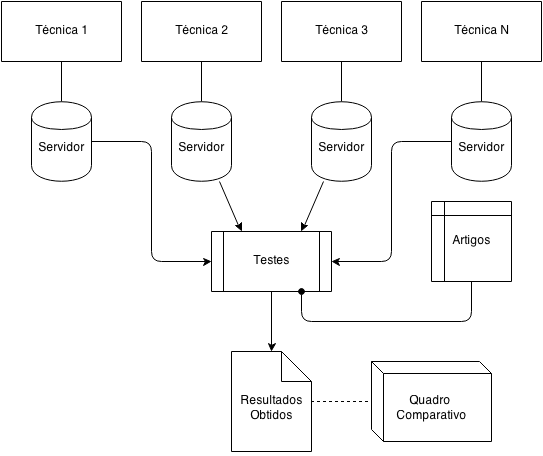
\includegraphics[width=0.8\linewidth]{./assets/images/metodology}
    \center\footnotesize{Fonte: O próprio autor}
\end{figure}


\section{Escolha do Corpus}
\label{sec:corpus}

% Falar da seleção de artigos de várias áreas

Visando verificar a eficiência das ferramentas - juntamente com a implementação das técnicas por elas utilizadas -, desejamos ter resultados precisos da extração de metadados, para que possam ser comparados e verificados com os metadados manualmente extraídos. Deste modo, foi selecionada uma série de artigos científicos das mais diversas áreas de pesquisa, com padrões visuais distintos.

% Porque selecionar artigos de diferentes áreas

Em virtude da necessidade de realizar testes em um ambiente real e representativo, foi realizada uma pesquisa no site do CNPq \url{http://www.cnpq.br/} para obter a relação das áreas e subáreas do conhecimento reconhecidas nacionalmente. Deste modo foi constatada a existência de 9 (nove) áreas do conhecimento, totalizando 1.290 (mil duzentas e noventa) subáreas, conforme pode ser verificado na \autoref{tab:areas-cnpq}.

\begin{table}[h!]
    \caption{Áreas do Conhecimento (CNPq)}
    \begin{center}
        \begin{tabular}{|l|c|}
            \hline 
            \textbf{Áreas do Conhecimento} & \textbf{Subáreas} \\ 
            \hline 
            Ciências Agrárias & 157 \\
            Ciências Biológicas & 104 \\
            Ciências da Saúde & 76 \\
            Ciências Exatas e da Terra & 243 \\
            Ciências Humanas & 163 \\
            Ciências Sociais Aplicadas & 185 \\
            Engenharias & 305 \\
            Linguística, Letras e Artes & 53 \\
            Outros & 4 \\
            \hline
            \textbf{Total} & \textbf{1290} \\
            \hline
        \end{tabular}
    \end{center}
    \center\footnotesize{Fonte: \url{http://www.memoria.cnpq.br/areasconhecimento/index.htm}}
    \label{tab:areas-cnpq}
\end{table}

Por causa do grande número de subdivisões de cada área do conhecimento (vide \autoref{tab:areas-cnpq}), a seleção das subáreas foi limitada a 2 (duas), sendo a escolha feita com base na existência de curso de graduação e/ou departamento na Universidade Federal de Minas Gerais (UFMG), o que facilitaria o contato com professores e coordenadores dos respectivos cursos. Desta forma, excluindo-se a área ``Outros'', seriam analisadas 16 (dezesseis) subáreas, sendo 2 (duas) para cada uma das 8 (oito) áreas do conhecimento.

Com as subáreas selecionadas, foi realizada uma entrevista com professores e/ou coordenadores de cada curso ou departamento correspondente na UFMG, obtendo então as bases de dados e/ou revistas mais utilizadas e relevantes para cada subárea do conhecimento, construindo um \emph{Corpus} realmente significativo.

Para cada uma destas subáreas do conhecimento foram coletados 7 (sete) artigos científicos. Em virtude da diversidade de bases de dados informadas pelos professores (\autoref{tab:databases}), a pesquisa foi limitada a 2 (duas) bases, na ordem apresentada pelos próprios pesquisadores, contemplando 4 (quatro) artigos para a primeira base e 3 (três) para a segunda. 

Para a subárea ``Ciências Biológicas (Genética)'' somente uma base de dados foi utilizada, portanto dela foram retirados todos os 7 artigos necessários. No total foram selecionados 112 (cento e doze) artigos, contemplando 16 (dezesseis) subáreas do conhecimento e 32 (trinta e duas) bases de dados, formando então o \emph{Corpus} utilizado nesta pesquisa.

\begin{table}[h!]
    \caption{Bases de Dados informadas pelos professores entrevistados, por subárea do conhecimento.}
    \begin{center}
        \begin{tabular}{|p{6cm}|p{8cm}|}
            \hline 
            \textbf{Subárea do Conhecimento} & \textbf{Bases de Dados} \\ 
            \hline 
            Arquitetura e Urbanismo & Scielo, Web of Science, Scopus \\
            \hline
            Ciência da Computação & DBLP, ACM Digital Library, IEEE Xplore \\
            \hline
            Ciência da Informação & LISA, ISTA, LISTA \\
            \hline
            Ciências Biológicas (Genética) & PubMed \\
            \hline
            Ciências Biológicas (Zoologia) & Zoological Records, Biological Abstracts \\
            \hline
            Enfermagem & MedLine, Lilacs, CINAHL, EBSCO, IBECS, BDENF \\
            \hline
            Engenharia Civil & Construction and Building Materials (ELSEVIER), Cement and Concrete Composites (ELSEVIER), Composites Science and Technology (ScienceDirect), Cement and Concrete Research (ELSEVIER), Materials Research (Scielo) \\
            \hline
            Engenharia Mecânica & Scopus, ScienceDirect, Web of Science, SpringerLink, Elsevier, Research Gate \\
            \hline
            Fonoaudiologia & Pubmed, Bireme \\
            \hline
            Geologia & Springer, Scielo, Portal CAPES \\
            \hline
            História & Scielo, Jstor, Redalyc \\
            \hline
            Letras & Delta (Scielo), Periódicos Letras UFMG, Periódicos UFSC \\
            \hline
            Medicina Veterinária & PubMed, Scielo \\
            \hline
            Música & RISM, RILM, JSTOR, Grove Dictionary of Music \\
            \hline
            Psicologia & Scopus, PsycInfo, Scopus, Psicodoc \\
            \hline
            Zootecnia & Dairy Science, Animal, Poultry Science \\
            \hline
        \end{tabular}
    \end{center}
    \label{tab:databases}
\end{table}

A seleção dos artigos em cada base de dados foi feita de maneira arbitrária, levando em consideração diferenças de leiautes e posicionamento dos elementos, permitindo que uma maior variedade de documentos fosse analisada.

% Artigos em Inglês, somente

Todos os artigos selecionados foram escritos na língua inglesa. Embora existam trabalhos locais relevantes para a área de extração de informação, esta decisão foi tomada por ser a língua mais utilizada no meio acadêmico, possuindo um universo muito maior de artigos escritos no idioma. Além disso, algumas das ferramentas e respectivas técnicas utilizam formas de ``processamento de linguagem natural'' para extração dos metadados, tendo por padrão a utilização do inglês na análise dos textos dos documentos de entrada.

Em virtude destas colocações a abrangência de outros idiomas entraria em um aspecto que não é objetivo deste trabalho abordar, visto a diversidade de culturas e símbolos, fazendo com que línguas orientais - como o mandarim ou japonês, por exemplo - tivessem análises diferenciadas em função de suas diferenças nas formas de representação e leitura, necessitando de outras técnicas e/ou ferramentas mais direcionadas para obter os resultados esperados.

Sobre a escolha das ferramentas para a realização dos testes foi utilizado apenas um critério na seleção: a sua utilização por linha de comando (\emph{command line}). Embora algumas ferramentas possuem código aberto a extração de metadados faz parte de um contexto específico da aplicação, dificultando a utilização somente deste recurso. Assim, foram selecionadas para testes apenas as ferramentas que permitem o uso de sua funcionalidade de extração de metadados de maneira individualizada, independente da linguagem de programação ou tecnologia apresentada. 

Assim, de acordo com os critérios adotados, as ferramentas selecionadas foram: Cermine, CiteSeer, CrossRef e ParsCit, como pode ser visto na \autoref{tab:selected-tools}.

\begin{table}[h!]
    \caption{Ferramentas selecionadas para o experimento.}
    \begin{center}
        \begin{tabular}{|C{3cm}|C{4cm}|C{6cm}|}
            \hline 
            \textbf{Ferramenta} & \textbf{Linguagens de Programação} & \textbf{Técnicas Utilizadas} \\ 
            \hline 
            Cermine & Java & SVM, CRF, Word Clustering \\ \hline
            CiteSeer & Python, Perl, Java & SVM, CRF (ParsCit), Word Clustering \\ \hline
            CrossRef & Ruby, Python & Expressões Regulares, Posicionamento Espacial \\ \hline
            ParsCit & Perl, Ruby & CRF \\ \hline
        \end{tabular}
    \end{center}
    \label{tab:selected-tools}
\end{table}
    
\section{Desenho do Experimento}
\label{sec:experiment-design}

Selecionadas as ferramentas e também os artigos que serão utilizados para os testes, parte-se para a instalação adequada de cada ferramenta, juntamente com as tecnologias necessárias e as linguagens de programação utilizadas pelos seus desenvolvedores. 

Cada ferramenta foi testada em separado, observando suas características particulares. Assim, cada artigo selecionado foi testado para cada uma das ferramentas, com os respectivos resultados de cada extração. Estes resultados foram separados por metadados, o que permitiu calcular qual a porcentagem de acerto que cada ferramenta obteve na extração de cada metadado analisado.

Assim, o processo foi repetido para cada ferramenta e o resultado registrado, permitindo calcular sua porcentagem total de acertos de maneira simplificada. Para isso foi criado um ``Quadro Comparativo'', no qual foram inseridos os resultados dos testes de cada ferramenta. 

No total foram analisados 112 (cento e doze) artigos científicos, para um total de 4 (quatro) ferramentas, totalizando 448 (quatrocentas e quarenta e oito) extrações de metadados através da linha de comando.

Todas as extrações foram feitas de forma automatizada, levando em consideração as necessidades de chamada de cada ferramenta, bem como os resultados de cada processamento para comparação. Todo o código criado pelo autor para este processo encontra-se disponível em \url{http://github.com/jgrossi/met}.

\subsection{Metadados, Pesos e Resultados}
\label{ssec:metadata-results}

% Importância de se ter pesos em função dos metadados

Em se tratando de pesquisa por artigos científicos, pequenos detalhes podem fazer diferença. Dessa forma, uma extração de metadados não muito eficaz pode prejudicar direta ou indiretamente os resultados da busca. Por outro lado, alguns metadados tendem a ser mais utilizados em pesquisas que outros, o que implica em uma responsabilidade maior na eficiência de sua extração. 

% Quais metadados são mais importantes para uma pesquisa de artigos

Geralmente quando vamos buscar artigos, procuramos primeiro pelo título - quando procuramos por um documento específico - ou então pelo nome do autor - quanto procuramos por artigos de um determinado pesquisador. Assim foram atribuídos pesos para cada um dos metadados, de maneira a valorizar essas informações que influenciam diretamente os resultados de busca.

A \autoref{tab:metadata-weight} mostra como cada metadado foi interpretado e qual o peso que lhe foi atribuído, sendo utilizado o inteiro 1 (um) para o peso mais baixo e o 5 (cinco) para o peso mais alto, sendo consequentemente o(s) metadado(s) mais importante(s) para uma pesquisa eficaz. Os pesos utilizados, assim como a ordem de importância escolhida se fundamentam apenas na experiência do autor.

% Tabela de metadados e pesos

\begin{table}[h!]
    \caption{Os metadados e seus pesos atribuídos}
    \begin{center}
        \begin{tabular}{|p{3cm}|p{8cm}|C{1cm}|}
            \hline \textbf{Metadado} & \textbf{Relevância} & \textbf{Peso} \\ 
            \hline Título & Um dos termos mais buscados quando se pesquisa um artigo & 5 \\
            \hline Autor(es) & Outro termo muito utilizado na busca por artigos & 4 \\
            \hline E-mail(s) & Pouco relevante no quesito pesquisa de artigos & 1 \\
            \hline Resumo & Importante por conter palavras chaves, além do resumo propriamente dito & 3 \\
            \hline Referências & Muito importante e necessário, pois será utilizada na referência inversa de autores & 4 \\
            \hline 
        \end{tabular} 
    \end{center}
    \label{tab:metadata-weight}
\end{table}

Como a extração de um metadado nem sempre ocorre de maneira 100\% eficaz, visando uma avaliação mais detalhada de cada ferramenta, foi calculada a precisão do resultado da extração de cada metadado, feita com base na porcentagem de sucesso obtida para aquele conjunto de caracteres. Este cálculo foi feito com o uso da função \texttt{similar\_text} da linguagem de programação PHP \url{http://php.net/similar_text}, que calcula a porcentagem de similaridade entre dois textos de acordo com o algoritmo proposto por Oliver \cite{oliver-1993}. Assim, foram comparados:

\begin{enumerate}
    \item O dado correto, retirado manualmente dos artigos, pelo próprio autor;
    \item O dado extraído, obtido por cada ferramenta.
\end{enumerate}

Esta taxa de acerto é referenciada posteriormente como, por exemplo, $P_{título}$ (porcentagem de acertos para o metadado título). Segundo a documentação da função \texttt{similar\_text} temos:

\begin{quote}
    \emph{``This calculates the similarity between two strings as described in Programming Classics: Implementing the World's Best Algorithms by Oliver (ISBN 0-131-00413-1). Note that this implementation does not use a stack as in Oliver's pseudo code, but recursive calls which may or may not speed up the whole process. Note also that the complexity of this algorithm is O(N**3) where N is the length of the longest string.''}
\end{quote}

Esta função recebe três parâmetros: o primeiro texto, o segundo texto e uma variável onde será armazenada a porcentagem de acerto. Como retorno tem-se um inteiro representando o número de caracteres comuns entre os dois textos comparados. Sua estrutura de utilização é a seguinte:

\lstset{language=PHP}
\begin{lstlisting}[escapechar=\#]
int similar_text ( string $first , string $second [, float &$percent ] )
\end{lstlisting}

Como cada ferramenta é testada em separado, os resultados da extração de cada artigo são gravados, tendo o total da precisão calculado de acordo com a média aritmética dos resultados obtidos para aquele metadado. Por exemplo, para a Ferramenta ``A'' foram analisados 100 (cem) artigos. A precisão na extração do título de cada artigo ($P_{título1}$, $P_{título2}$, ..., $P_{títuloN}$), por exemplo, é somada e o resultado dividido pelo número de artigos - no caso 100. Assim tem-se a precisão geral para o metadado ``Título'' para a Ferramenta ``A'' ($P_{título}$):

\begin{center}
    \begin{math}
        P_{título} = (P_{título1} + P_{título2} + P_{título3} ... + P_{título100}) / 100
        \label{math:result-by-metadata}
    \end{math}
\end{center}

De posse dos acertos de cada metadado extraído podemos comparar os resultados de cada ferramenta, permitindo conclusões sobre o comportamento de cada uma perante cada metadado. Espera-se poder inferir, portanto, que a ferramenta ``X'' apresenta melhores resultados do que ``Y'' na extração do nome dos autores, por exemplo.

\subsection{Índice de Confiabilidade}
\label{ssec:confiability-index}

% Fórmula final para a nota final de cada técnica

Considerando que cada metadado possui um peso diferente (vide \autoref{tab:metadata-weight}) é necessário calcular o índice de acertos com base nos resultados obtidos por cada ferramenta, para cada metadado. Assim chegou-se a uma fórmula matemática nomeada ``Índice de Confiabilidade'', que calcula o resultado obtido através dos pesos que foram atribuídos a cada metadado, para cada ferramenta. 

Este índice é a nota final de cada ferramenta, levando em consideração todos os resultados obtidos por ela para os artigos utilizados neste trabalho. Nele são empregados os pesos anteriormente definidos e a precisão dos resultados, permitindo chegar a uma única nota para cada ferramenta testada.

Esta fórmula é a média ponderada dos resultados alcançados na extração de cada metadado dos artigos, seguindo os pesos apresentados na \autoref{tab:metadata-weight}. Cada peso é atribuído ao resultado encontrado em cada ferramenta. 

A título de exemplo, após o teste de uma ferramenta, supondo que ela conseguiu extrair 87\% dos títulos de todos os artigos com sucesso, sua precisão com relação ao título será 87 ($P_{título}=87$), que será multiplicada pelo peso correspondente, neste caso, o inteiro 5. Isso ocorre para todos os metadados extraídos, seguindo seus respectivos pesos. A descrição de cada variável do Índice de Confiabilidade é apresentada na \autoref{tab:confiability-index}.

\begin{center}
    $ IC_{Ferramenta X}=(5*P_{título}+4*P_{autor}+1*P_{email}+3*P_{resumo}+4*P_{referências}) / 17 $
\end{center}

\begin{table}[h!]
    \caption{Descrição de cada variável no Índice de Confiabilidade}
    \begin{center}
        \begin{tabular}{|p{3cm}|p{8cm}|}
            \hline \textbf{Variável} & \textbf{Descrição}\\ 
            \hline $P_{título}$ & Precisão na obtenção do título \\
            \hline $P_{autor}$ & Precisão na obtenção do(s) autor(es)\\
            \hline $P_{email}$ & Precisão na obtenção dos e-mails dos autores \\
            \hline $P_{resumo}$ & Precisão na obtenção do resumo \\
            \hline $P_{referências}$ & Precisão na obtenção das referências \\
            \hline 
        \end{tabular} 
    \end{center}
    \label{tab:confiability-index}
\end{table}

Assim, de posse do Índice de Confiabilidade de cada ferramenta podemos classificá-las com base em seus resultados. Esta classificação não tem por objetivo qualquer favorecimento de ferramentas, mas sim classificar cada uma delas com base nos resultados obtidos e critérios adotados neste trabalho. Desta forma, cada ferramenta foi classificada seguindo os valores abaixo:

\begin{enumerate}
    \item \textbf{Precisa (P):} Quando o Índice de Confiabilidade é maior ou igual a 80 ($IC\geq80$).
    \item \textbf{Satisfatória (S):} Quando o Índice de Confiabilidade é maior ou igual a 60 e menor que 80 ($60 \leq IC < 80$).
    \item \textbf{Insatisfatória (I):} Quando o Índice de Confiabilidade é menor que 60 ($IC < 60$).
\end{enumerate}

\section{Ambiente Tecnológico}
\label{sec:tech-environment}

As ferramentas testadas - por utilizarem das mesmas linguagens de programação ou por terem seus conjuntos tecnológicos semelhantes - foram instaladas em um único servidor, permitindo também que recursos computacionais fossem compartilhados, simplificando o trabalho de configuração em função de necessidades parecidas.

Este servidor foi criado através de máquina virtual, o que traz benefícios não somente de performance mas de flexibilidade quanto às tecnologias necessárias para o correto funcionamento de cada ferramenta. Este fato permitiu que os testes fossem feitos em sistemas operacionais distintos porém utilizando os mesmos recursos computacionais da máquina de origem.


